\documentclass[11pt, a4paper]{article}

\usepackage[T1]{fontenc}
\usepackage[utf8]{inputenc}
\usepackage{amsmath, amssymb, amsthm}
\usepackage{geometry}
\usepackage{booktabs}
\usepackage{enumitem}
\usepackage{hyperref}
\usepackage{xcolor}
\usepackage{titlesec}
\usepackage{parskip}
\usepackage{tikz}
\usepackage{pgfplots}
\pgfplotsset{compat=1.18}

\geometry{margin=2.5cm}

\hypersetup{
  colorlinks=true,
  linkcolor=blue!60!black,
  urlcolor=blue!60!black
}

\titleformat{\section}{\large\bfseries}{\thesection.}{0.6em}{}[\titlerule]
\titleformat{\subsection}{\normalsize\bfseries}{\thesubsection}{0.6em}{}

\title{\textbf{Model Validation Interview Preparation}\\[0.4em]
\large A Question List, with a Worked Discussion of the Kolmogorov--Smirnov Test\\[0.2em]
\normalsize v13 --- May 2026}
\author{}
\date{}

\begin{document}
\maketitle
{\small\tableofcontents}

\clearpage

%=============================================================
\section{About this document}
%=============================================================

A friend who works in model validation at a Canadian bank walked me
through the question list he uses when interviewing MV candidates,
and encouraged me to publish my notes from that conversation.  Here
they are.

The format is simple: I went down the list and wrote up the items
that either interested me or that I felt I should know better.  The
Kolmogorov--Smirnov test (Section 9) got the most attention because
my own understanding of it was the weakest going in.  Other items
are sketched lightly, sometimes only as a paragraph.  Whether a
topic gets one paragraph or six pages reflects where I happened to
have a gap, not the topic's importance.

What is most likely to come next is a fuller treatment of
homoscedasticity --- the assumption itself and the Breusch--Pagan
test for it --- which is what I am working on right now.

If you spot a mistake or want to add a discussion of your own,
open an issue at
\url{https://github.com/borisgarbuzov/notes} or comment on the
LinkedIn post.

%=============================================================
\section{Overview: MV Specializations}
%=============================================================

Model validation (MV) roles vary significantly by the type of model being validated.
The main domains and their primary modelling paradigms are:

\begin{center}
\begin{tabular}{lll}
\toprule
\textbf{Domain} & \textbf{Model type} & \textbf{Key techniques} \\
\midrule
Credit Risk & Regression / scoring & PD, LGD, EAD models; logistic regression \\
Stress Testing & Macro-conditional regression & OSFI/DFAST scenarios; satellite models \\
Fraud Detection & Classification & Logistic, random forest, XGBoost \\
AML & Unsupervised learning & Clustering, anomaly detection \\
Option Pricing / Market Risk & Stochastic processes & BSM, Monte Carlo, Greeks \\
Treasury / ALM & Interest rate models & Duration, convexity, gap analysis \\
\bottomrule
\end{tabular}
\end{center}

\textit{Credit Risk and Stress Testing were flagged as the highest-priority domains for preparation.}

%=============================================================
\section{Linear Regression: Assumptions and Violations}
%=============================================================

\subsection{The Classical Assumptions (Gauss-Markov)}

Let the model be $Y = X\beta + \varepsilon$.

\begin{enumerate}[label=\textbf{(\alph*)}]

\item \textbf{Linearity.}
The relationship between $Y$ and each regressor is linear.
\textit{Diagnostic:} scatter plots of $Y$ vs.\ each $X_j$; residual-vs-fitted plot.

\item \textbf{No multicollinearity.}
The regressors are not perfectly (or near-perfectly) linearly dependent.
\textit{Diagnostic:} Variance Inflation Factor
\[
  \mathrm{VIF}_j = \frac{1}{1 - R^2_j},
\]
where $R^2_j$ is the $R^2$ from regressing $X_j$ on all other regressors.
Rule of thumb: $\mathrm{VIF} > 10$ signals a problem.

\item \textbf{No autocorrelation of residuals.}
$\mathrm{Cov}(\varepsilon_i, \varepsilon_j) = 0$ for $i \neq j$.
\textit{Diagnostic:} \textbf{Durbin-Watson} statistic
\[
  DW = \frac{\sum_{t=2}^{n}(\hat\varepsilon_t - \hat\varepsilon_{t-1})^2}{\sum_{t=1}^n \hat\varepsilon_t^2}.
\]
$DW \approx 2$ indicates no autocorrelation; $DW < 2$ positive, $DW > 2$ negative autocorrelation.

\item \textbf{Residuals are normally distributed with zero mean.}
$\varepsilon \sim N(0, \sigma^2 I)$.
\textit{Diagnostics:}
\begin{itemize}
  \item Zero-mean: one-sample $t$-test on residuals.
  \item Normality: \textbf{Kolmogorov-Smirnov (KS) test}; also Shapiro-Wilk, Q-Q plot.
\end{itemize}

\item \textbf{Homoscedasticity.}
$\mathrm{Var}(\varepsilon_i) = \sigma^2$ (constant variance).

\textbf{Theoretical basis (from first principles).}
Write the model as $y = \beta_0 + \beta_1 x + \varepsilon$ with $\mathbb{E}\varepsilon = 0$.
Introduce an auxiliary model for the variance:
\[
  \varepsilon^2 = h(\alpha_0 + \alpha_1 x) + u, \quad
  \mathbb{E}u = 0,\quad \mathbb{E}(u|x) = 0 \text{ a.s.}
\]
Then:
\[
  \mathrm{Var}(\varepsilon|x)
  = \mathbb{E}(\varepsilon^2|x)
  = \mathbb{E}(h(\alpha_0+\alpha_1 x)+u\mid x)
  = h(\alpha_0+\alpha_1 x) + 0
  = h(\alpha_0+\alpha_1 x).
\]
Homoscedasticity by definition means $\mathrm{Var}(\varepsilon|x) = \text{const}$,
i.e.\ $h(\alpha_0+\alpha_1 x) = \text{const}$.
A natural sufficient condition is $\alpha_1 = 0$.
The \textbf{Breusch--Pagan test} tests exactly this:
\[
  H_0\colon \alpha_1 = 0.
\]

\textit{Diagnostic procedure:} regress $\hat\varepsilon^2$ on the regressors;
the test statistic $nR^2 \sim \chi^2_k$ under $H_0$.

\end{enumerate}

\subsection{Consequences of Violations}

\begin{enumerate}[label=\textbf{(\alph*)}]

\item \textit{Multicollinearity violated:}
$\hat\beta$ remains unbiased but is \textbf{no longer consistent} in the sense that $\hat\beta \to \Sigma$ (the coefficient estimates are unstable and highly sensitive to small changes in data). Standard errors are inflated; interpretation of individual coefficients is meaningless.

\item \textit{Autocorrelation or heteroscedasticity violated (assumptions c and e):}
$\hat\beta$ is still unbiased, but $\widehat{\mathrm{Var}}(\hat\beta)$ is \textbf{incorrect}, invalidating all $t$- and $F$-tests.
\textit{Remedy:} use \textbf{Newey-West} (HAC) standard errors, which are robust to both autocorrelation and heteroscedasticity without re-specifying the model.

\end{enumerate}

%=============================================================
\section{Logistic Regression: Assumptions}
%=============================================================

Logistic regression models the probability of a binary outcome:
\[
  P(Y=1 \mid X) = \frac{1}{1 + e^{-X\beta}} = \sigma(X\beta).
\]

Key assumptions:
\begin{enumerate}[label=\textbf{(\alph*)}]
\item \textbf{Binary (or ordinal) outcome.} The dependent variable must be categorical.
\item \textbf{No multicollinearity} among regressors (same as linear regression; check VIF).
\item \textbf{Independence of observations.}
\item \textbf{Large sample size} (MLE relies on asymptotic theory).
\item \textbf{No extreme outliers} (influential observations distort MLE).
\end{enumerate}

Note: logistic regression does \emph{not} require normality of residuals or homoscedasticity.

%=============================================================
\section{Hypothesis Testing: Core Concepts}
%=============================================================

\subsection{Type I and Type II Errors}

\begin{center}
\begin{tabular}{lcc}
\toprule
 & $H_0$ true & $H_0$ false \\
\midrule
Reject $H_0$ & \textbf{Type I error} ($\alpha$) & Correct (Power) \\
Fail to reject $H_0$ & Correct & \textbf{Type II error} ($\beta$) \\
\bottomrule
\end{tabular}
\end{center}

\begin{itemize}
  \item \textbf{Type I error} (false positive): reject $H_0$ when it is true. Probability $= \alpha$ (significance level).
  \item \textbf{Type II error} (false negative): fail to reject $H_0$ when it is false. Probability $= \beta$.
\end{itemize}

\subsection{p-value}

The \textbf{p-value} is the probability of observing a test statistic at least as extreme as the one computed, \emph{under the assumption that $H_0$ is true}:
\[
  p = P(T \geq t_{\mathrm{obs}} \mid H_0).
\]
A small $p$-value (typically $< \alpha = 0.05$) is evidence against $H_0$. The p-value is \emph{not} the probability that $H_0$ is true.

\subsection{Statistical Power}

\[
  \text{Power} = 1 - \beta = P(\text{reject } H_0 \mid H_0 \text{ is false}).
\]
Power increases with: larger sample size $n$, larger effect size, lower $\sigma$, higher $\alpha$.

%=============================================================
\section{Probability: Foundational Definitions}
%=============================================================

\subsection{Marginal and Conditional Probability}

\begin{itemize}
  \item \textbf{Marginal probability:} $P(A)$ --- the probability of event $A$ regardless of any other event.
  \item \textbf{Conditional probability:}
  \[
    P(A \mid B) = \frac{P(A \cap B)}{P(B)}, \quad P(B) > 0.
  \]
  \item \textbf{Multiplication rule:}
  \[
    P(A \cap B) = P(A \mid B)\,P(B) = P(B \mid A)\,P(A).
  \]
\end{itemize}

\subsection{Law of Total Probability}

If $\{B_1, B_2, \ldots, B_n\}$ is a partition of the sample space (mutually exclusive and exhaustive), then
\[
  P(A) = \sum_{i=1}^{n} P(A \mid B_i)\,P(B_i).
\]

\subsection{Independence}

Events $A$ and $B$ are \textbf{independent} if and only if any of the following equivalent conditions holds:
\[
  P(A \mid B) = P(A), \qquad P(B \mid A) = P(B), \qquad P(A \cap B) = P(A)\,P(B).
\]

\subsection{Integration Using the Kernel of a PDF}

A useful technique: identify the \emph{kernel} of a known distribution inside an integral and use the fact that the PDF integrates to 1.

\textbf{Example --- Normal PDF.}
\[
  f(x \mid \mu, \sigma^2) = \frac{1}{\sqrt{2\pi}\,\sigma}\,\exp\!\left(-\frac{(x-\mu)^2}{2\sigma^2}\right).
\]
The \emph{kernel} is $\exp\!\bigl(-(x-\mu)^2 / (2\sigma^2)\bigr)$.

\textbf{Classic interview integral:} Evaluate
\[
  I = \int_{-\infty}^{\infty} e^{-\left(\frac{x-\mu}{\sigma}\right)^2} dx.
\]
\textit{Solution.} Write $u = (x-\mu)/\sigma$, $dx = \sigma\,du$:
\[
  I = \sigma \int_{-\infty}^{\infty} e^{-u^2} du = \sigma\sqrt{\pi}.
\]
The last step uses the Gaussian integral $\int_{-\infty}^{\infty} e^{-u^2}du = \sqrt{\pi}$.

More generally, since $\int_{-\infty}^{\infty} f(x\mid\mu,\sigma^2)\,dx = 1$:
\[
  \int_{-\infty}^{\infty} e^{-(x-\mu)^2/(2\sigma^2)}\,dx = \sqrt{2\pi}\,\sigma.
\]

%=============================================================
\section{Structure of a Model Validation Project}
%=============================================================

The typical deliverables of an MV engagement are:

\begin{enumerate}[label=\textbf{\arabic*.}]

\item \textbf{Data replication.}
Independently reproduce the training/calibration dataset from source systems.
Verify row counts, distributions, and key statistics across time periods.
\textit{Example:} model developer reports 2025 Q1 portfolio = \$1.0M, 2025 Q2 = \$0.8M.
Validator independently reconstructs both figures; unexplained gap of $-\$0.2$M triggers investigation.

\item \textbf{Model replication.}
Re-implement the model independently (or re-run developer code) to reproduce reported outputs: coefficients, predictions, performance metrics.
Discrepancies indicate either data or implementation errors.

\item \textbf{Assumption checks.}
Formally test all model assumptions as per the validation guideline (e.g.\ OSFI E-23, SR 11-7).
For regression models: linearity, no multicollinearity, no autocorrelation, normality, homoscedasticity (see Section 2).

\item \textbf{Backtesting.}
Compare model predictions against actual realised outcomes on out-of-time or out-of-sample data.
\textit{Metrics:} Gini coefficient, AUC-ROC, KS statistic (for credit), RMSE/MAE (for regression), PSI for population stability.

\item \textbf{Benchmarking.}
Compare the validated model against one or more challenger models.
\textit{Process:} model developers typically present a set of candidate models (e.g.\ models a, b, c, d, e) and select a champion.
The validator independently constructs a benchmark (possibly a subset or alternative ranking, e.g.\ b, d, g, e, c) to assess whether the champion selection is defensible.

\item \textbf{Challenges / findings.}
Document material findings, assign risk ratings (low / medium / high), and issue recommendations or conditions on model use.

\end{enumerate}

%=============================================================
\section{Foundations of Statistical Testing}
%=============================================================

This section sets out the mathematical skeleton of hypothesis testing before applying
it to specific tests (Breusch--Pagan, KS).  The observations below revisit material from
graduate-level theoretical statistics in language adapted to the validation context.

\subsection{A Test Is a Bernoulli-Valued Statistic}

Let $(\Omega, \mathcal{F}, \{P_\theta\}_{\theta\in\Theta})$ be a statistical model.
A \textbf{test} is any measurable function
\[
  \phi: \mathcal{X} \to \{0, 1\},
\]
where $\mathcal{X}$ is the sample space ($\phi=1$ means reject $H_0$, $\phi=0$ means
do not reject). This is the minimal definition: no further structure is required.

\textbf{Remark on randomised tests.}
One sometimes allows $\phi:\mathcal{X}\to[0,1]$, interpreted as the probability of
rejection given the observed sample. This is needed to achieve an exact size $\alpha$
in discrete models (e.g.\ binomial). The Neyman--Pearson lemma in its full generality
requires randomised tests. In practice they are rarely used.

\textbf{Trivial tests.}
$\phi\equiv 0$ (never reject) has $\alpha=0$, $\beta=1$.
$\phi\equiv 1$ (always reject) has $\alpha=1$, $\beta=0$.
Both are formally valid tests. Their existence shows that the Bernoulli property alone
says nothing useful: we need additional constraints.

\subsection{Type I and II Errors; the Partial Order on Tests}

For a test $\phi$ and hypotheses $H_0$, $H_1$:
\[
  \alpha(\phi) = \sup_{\theta\in H_0} E_\theta[\phi(X)], \qquad
  \beta(\phi)  = \sup_{\theta\in H_1} E_\theta[1-\phi(X)].
\]
$\alpha$ is the \textbf{size} (worst-case Type~I error rate),
$\beta$ is the worst-case Type~II error rate, and $1-\beta$ is the \textbf{power}.

Tests are partially ordered: $\phi_1$ \emph{dominates} $\phi_2$ if
$\alpha(\phi_1)\leq\alpha(\phi_2)$ and $\beta(\phi_1)\leq\beta(\phi_2)$, with at least
one strict. Most pairs of tests are incomparable in this order --- one has smaller
$\alpha$, the other smaller $\beta$.

\textbf{Standard resolution (Neyman--Pearson paradigm).}
Fix a tolerated Type~I error $\alpha_0$ (typically 0.05) and minimise $\beta$ within
the class $\{\phi: \alpha(\phi)\leq\alpha_0\}$.
This resolves incomparability by making $\alpha$ the primary constraint and $\beta$
the objective. The asymmetry is conventional, not mathematical:\ $H_0$ plays the role
of the status quo, and the industry assigns it 95\% survival against a challenger $H_1$
that must overcome the 5\% hurdle.

\textbf{Alternative: Bayesian weighting.}
Assign prior probabilities $\pi_0, \pi_1$ to $H_0, H_1$ and costs $c_{01}, c_{10}$
to each error type. Minimise $\pi_0 c_{01}\alpha + \pi_1 c_{10}\beta$.
This gives a different optimal threshold and resolves incomparability differently.
The Neyman--Pearson approach is the frequentist special case with $\pi_0 c_{01} = \pi_1 c_{10}$
(symmetric costs) and hard constraint replacing soft penalty.

\subsection{Simple vs.\ Composite Hypotheses}

A \textbf{simple hypothesis} is a single measure: $H_0 = \{P_0\}$.
A \textbf{composite hypothesis} is a set of measures: $H_0 = \{P_\theta: \theta\in\Theta_0\}$.

For \emph{two simple hypotheses}, the Neyman--Pearson lemma gives the optimal test:
threshold the likelihood ratio $\Lambda(x) = \frac{dP_1}{dP_0}(x)$ at some $c$.
It exists, is essentially unique, and achieves maximum power at level $\alpha$.

For composite hypotheses, $\Lambda$ is no longer well-defined (which $P_1$ do you use?).
The best general outcome is a \textbf{uniformly most powerful (UMP)} test: one that
maximises power against every $\theta\in H_1$ simultaneously at level $\alpha_0$.
UMP tests exist only in special cases --- primarily one-parameter exponential families
with monotone likelihood ratio (one-sided testing). In most multiparameter or two-sided
problems, UMP does not exist, and one resorts to:
\begin{itemize}
  \item \textbf{UMPU}: uniformly most powerful among unbiased tests.
  \item \textbf{LRT}: likelihood ratio test --- maximise $\sup_{H_1} L$ vs.\
        $\sup_{H_0} L$; asymptotically optimal under regularity conditions.
  \item \textbf{Traditional statistics}: $t$, $F$, $\chi^2$, derived from pivotal
        quantities and validated by experience.
\end{itemize}

\subsection{The Role of $\Omega$ and the Sample Size $n$}

The probability space $(\Omega,\mathcal{F},P)$ is abstract. In practice we observe
$X:\Omega\to\mathcal{X}$, and the test lives on $\mathcal{X}$.
The connection to $\Omega$ is implicit.

A subtlety often swept under the rug: for a fixed statistic $T$ (say, the sample mean),
each sample size $n$ gives a \emph{different} test $\phi_n$. Properties such as
consistency and power are properties of the \emph{sequence} $\{\phi_n\}_{n\geq 1}$,
not of a single test.

\subsection{p-value: Definition and Limitations}

The \textbf{p-value} is informally ``the probability of observing an outcome at least as
extreme as the one observed, under $H_0$.'' Formally:
\[
  p(x) = \sup_{\theta\in H_0} P_\theta\bigl(T(X) \geq T(x)\bigr),
\]
where $T$ is a scalar test statistic and ``$\geq$'' encodes the ordering of outcomes
by their evidence against $H_0$.

This definition requires:
\begin{enumerate}[label=(\roman*)]
  \item A scalar statistic $T$ with a known (or parameter-free) distribution under $H_0$.
  \item A sensible ordering: large values of $T$ are more adverse to $H_0$.
        This ordering is a partial order on outcomes; without it, ``at least as extreme''
        is undefined.
  \item The distribution of $T$ under $H_0$ to be the same for all $\theta\in H_0$
        (pivotal quantity), otherwise the $\sup$ may be a conservative bound only.
\end{enumerate}

\textbf{When p-value is well-defined and exact.}
The KS test is the cleanest example: $T = D_n$ has the same distribution $G_n$ for
\emph{every} continuous $F_0$ at every finite $n$ (distribution-free property).
No $\sup$ is needed; the p-value is exact.

\textbf{When p-value is approximate or ill-defined.}
For composite $H_0$ with nuisance parameters, $P_\theta(T \geq t)$ depends on $\theta$,
and one takes the $\sup$, yielding a conservative p-value.
In high-dimensional or nonparametric settings, there may be no natural scalar $T$,
and the p-value loses a clean interpretation.

\textbf{An observation worth flagging: ``further from $H_0$'' $\not\Rightarrow$ ``closer to $H_1$.''}
The natural metric on the parameter space may not align with the power direction.
A test optimal for detecting deviations in all directions simultaneously (e.g.\ a
two-sided $t$-test) is suboptimal against a one-sided alternative.
Conversely, a one-sided test has no power against the opposite direction.
This is not a defect but a fundamental feature: without specifying $H_1$, there is no
universally best direction of extremeness.

\subsection{Consistency of a Test Sequence}

A sequence of tests $\{\phi_n\}$ at fixed level $\alpha$ is \textbf{consistent} against
$H_1$ if the power $1-\beta_n \to 1$ as $n\to\infty$ for every $\theta\in H_1$.

\textbf{Clarification on the joint behaviour of $\alpha$ and $\beta$.}
Simultaneously driving both $\alpha_n\to 0$ and $\beta_n\to 0$ is possible if one
relaxes the fixed-level constraint. For example, setting $\alpha_n = n^{-1/2}$ and
raising the threshold accordingly can yield $\beta_n\to 0$ as well. But this is
non-standard. The classical framework fixes $\alpha$ and asks only that $\beta_n\to 0$:
consistency is a one-sided guarantee.

The reason for the asymmetry mirrors the earlier one: $\alpha$ is a hard constraint
(we do not want to exceed the nominal false positive rate), while $\beta$ is an
objective (we want power, and we accept that more data is needed for harder alternatives).

\subsection{Pivotal Quantities and the Traditional Test Statistic}

A \textbf{pivotal quantity} is a function of the data and parameter whose distribution
under $H_0$ does not depend on any unknown parameter.
Examples: $\frac{\bar X - \mu_0}{S/\sqrt{n}} \sim t_{n-1}$ (Student's $t$, exact);
$\sqrt{n}\,D_n \to K$ (KS, asymptotically pivotal).

When a pivot exists, it is natural to use it as the test statistic, because:
\begin{itemize}
  \item Its null distribution is known --- no simulation or bootstrap needed.
  \item The p-value is exact (or asymptotically exact).
  \item Critical values can be tabulated once.
\end{itemize}

The Bernoulli test statistic $\phi = \mathbf{1}[T > c_\alpha]$ is the final step.
Tradition calls $T$ ``the test statistic'' even though $\phi$ is the actual test.
When no pivot exists, one still gets a Bernoulli test (e.g.\ via simulation), but the
intermediate scalar $T$ does not have the same clean properties.

%=============================================================
\section{The Kolmogorov-Smirnov Test}
%=============================================================

% ---- 7.1 The fundamental fact ----
\subsection{The Fundamental Fact: Distribution-Free Property}

\textit{(This characterisation of the KS test as exactly distribution-free at every
finite $n$ comes from re-reading Kolmogorov's original 1933/1941 paper in the course
of preparing these notes; it is rarely emphasised in textbooks, which usually present
only the asymptotic Kolmogorov-distribution result.)}

\medskip
The entire KS test rests on one remarkable observation.

\begin{quote}
\textbf{Theorem (Kolmogorov 1933).}
Let $X_1,\ldots,X_n\overset{\text{iid}}{\sim}F$ where $F$ is \emph{any} continuous CDF.
Then the distribution of
$D_n = \sup_x |F_n(x) - F(x)|$
does \textbf{not depend on} $F$.
\end{quote}

\textbf{Proof sketch.}
The probability integral transform gives $U_i = F(X_i) \sim \mathrm{Uniform}(0,1)$.
Applying $F$ to every observation maps the original sample to a uniform sample, and
$D_n$ computed against $F$ equals $D_n$ computed for the uniform sample against
$\mathrm{Uniform}(0,1)$.
The distribution of the latter depends only on $n$.

\textbf{Why this is stronger than the asymptotic statement.}
The theorem says that for \emph{every fixed} $n$, the distribution $G_n$ of $D_n$ is
the same for all continuous $F$.
This is not just a statement about the limit $n\to\infty$: it holds exactly at $n=5$,
$n=10$, $n=100$, or any other sample size.

\textbf{Consequences.}
\begin{itemize}
  \item \textbf{Exact tabulation for any $n$.}
        Because $G_n$ is universal, it can be computed once and tabulated.
        This is the origin of the exact critical values $D_{n,\alpha}$
        (double-indexed by $n$ and significance level $\alpha$):
        \[
          P_{H_0}(D_n > D_{n,\alpha}) = \alpha,
        \]
        the same equation for every continuous $F_0$.
  \item \textbf{Asymptotic regime.}
        As $n\to\infty$, $G_n$ converges to the Kolmogorov distribution $G$
        (Theorem~2 below), giving the large-sample formula.
  \item \textbf{Discontinuous $F_0$.}
        If $F_0$ is not continuous, $D_n$ depends on $F_0$.
        However, Kolmogorov (1941, Theorem~3) showed
        $P(D_n \leq \lambda) \geq G_n(\lambda)$ for all $\lambda$,
        so the test remains conservative.
\end{itemize}

\textit{A note on the source.}
``Confidence Limits for an Unknown Distribution Function,''
\textit{Annals of Math.\ Stat.}, 1941, is three pages without proofs --- a short
communication summarising Kolmogorov's 1933 Italian paper
(\textit{Giornale dell'Istituto Italiano degli Attuari}).
Theorem~2 states convergence ``uniformly in $\lambda$'' with no domain restriction;
as our partial-sum analysis shows, convergence holds for $\lambda>0$ only
(at $\lambda=0$ the partial sums oscillate between 0 and 2).
Read it as an authoritative reference card, not a self-contained proof.

% ---- 7.2 The two convergence theorems ----
\subsection{Two Convergence Results}

\textbf{Theorem 1 (Glivenko--Cantelli).}
\[
  \sup_x |F_n(x) - F(x)| \xrightarrow{a.s.} 0.
\]
Pointwise convergence follows from the LLN; the theorem strengthens it to
\emph{uniform} convergence: for almost all $\omega$, the whole staircase $F_n$
converges to $F$ as a function.

\textbf{Theorem 2 (Kolmogorov--Smirnov).}
\[
  \sqrt{n}\,D_n \xrightarrow{d} K, \qquad
  K = \sup_{t\in[0,1]}|B_t|, \quad B_t = W_t - t W_1\ (\text{Brownian bridge}).
\]
The factor $\sqrt{n}$ compensates the $O(1/\sqrt{n})$ rate from Theorem~1.
The limiting distribution $K$ is the \textbf{Kolmogorov distribution}: parameter-free,
defined via the Brownian bridge.

\textbf{Survival function of $K$.}
Two complementary series (both valid for $t>0$, related by the Jacobi theta identity):
\begin{align*}
  P(K \geq t) &= 2\sum_{k=1}^{\infty}(-1)^{k-1}e^{-2k^2t^2}
    && \text{(fast for large }t\text{)} \\
  P(K \leq x) &= \frac{\sqrt{2\pi}}{x}\sum_{k=1}^{\infty}e^{-(2k-1)^2\pi^2/(8x^2)}
    && \text{(fast for small }x\text{)}
\end{align*}
For $t \geq 1.2$ the first term of Series~A alone is accurate to $10^{-4}$.

\textbf{Partial sums and monotonicity.}
Individual partial sums of Series~A are not survival functions.
Odd-$N$ truncations ($N=1,3,5,\ldots$) start near 2 near the origin and decrease
monotonically; even-$N$ truncations ($N=2,4,6,\ldots$) start near 0, rise to a hump,
then decrease.
As $N\to\infty$ the hump migrates toward $t=0$; convergence is on $(0,\infty)$
only (at $t=0$ the series diverges).

\begin{center}
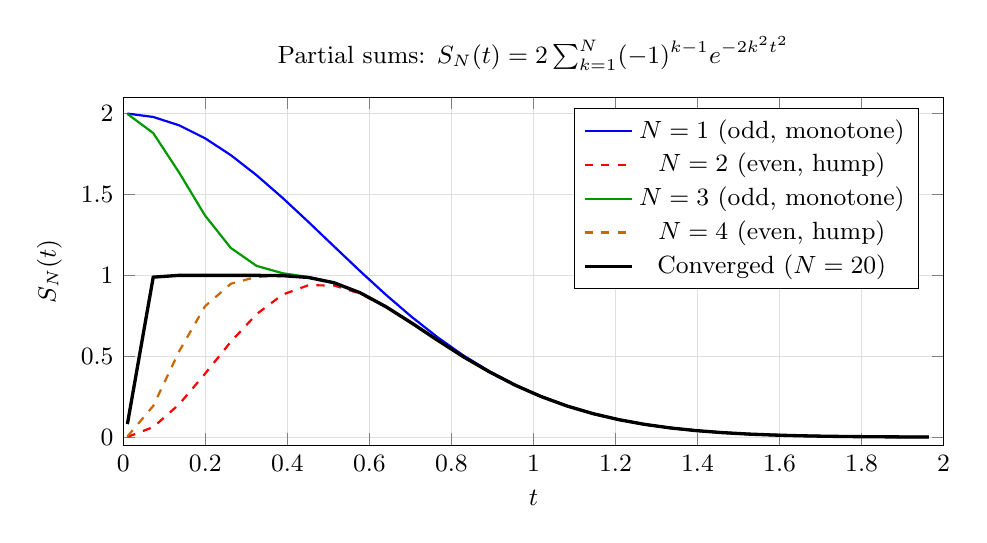
\begin{tikzpicture}
\begin{axis}[
  width=12cm, height=6cm,
  xlabel={$t$}, ylabel={$S_N(t)$},
  xmin=0, xmax=2.0, ymin=-0.05, ymax=2.1,
  grid=major, grid style={gray!25},
  legend pos=north east, legend style={font=\small},
  tick label style={font=\small}, label style={font=\small},
  title style={font=\small},
  title={Partial sums: $S_N(t)=2\sum_{k=1}^{N}(-1)^{k-1}e^{-2k^2t^2}$}
]
\addplot[blue,thick,solid] coordinates {(0.010,1.9996)(0.073,1.9788)(0.136,1.9273)(0.199,1.8475)(0.262,1.7432)(0.325,1.6187)(0.388,1.4795)(0.451,1.3309)(0.514,1.1784)(0.577,1.0269)(0.640,0.8807)(0.703,0.7435)(0.766,0.6177)(0.829,0.5051)(0.893,0.4065)(0.956,0.3220)(1.019,0.2511)(1.082,0.1927)(1.145,0.1455)(1.208,0.1082)(1.271,0.0791)(1.334,0.0570)(1.397,0.0404)(1.460,0.0282)(1.523,0.0193)(1.586,0.0131)(1.649,0.0087)(1.712,0.0057)(1.775,0.0037)(1.838,0.0023)(1.901,0.0015)(1.964,0.0009)};
\addlegendentry{$N=1$ (odd, monotone)}
\addplot[red,thick,dashed] coordinates {(0.010,0.0012)(0.073,0.0623)(0.136,0.2027)(0.199,0.3911)(0.262,0.5890)(0.325,0.7605)(0.388,0.8806)(0.451,0.9387)(0.514,0.9374)(0.577,0.8879)(0.640,0.8055)(0.703,0.7053)(0.766,0.5995)(0.829,0.4970)(0.893,0.4031)(0.956,0.3207)(1.019,0.2506)(1.082,0.1925)(1.145,0.1455)(1.208,0.1082)(1.271,0.0791)(1.334,0.0570)(1.397,0.0404)(1.460,0.0282)(1.523,0.0193)(1.586,0.0131)(1.649,0.0087)(1.712,0.0057)(1.775,0.0037)(1.838,0.0023)(1.901,0.0015)(1.964,0.0009)};
\addlegendentry{$N=2$ (even, hump)}
\addplot[green!60!black,thick,solid] coordinates {(0.010,1.9976)(0.073,1.8792)(0.136,1.6358)(0.199,1.3708)(0.262,1.1695)(0.325,1.0586)(0.388,1.0133)(0.451,0.9899)(0.514,0.9545)(0.577,0.8928)(0.640,0.8068)(0.703,0.7055)(0.766,0.5995)(0.829,0.4970)(0.893,0.4031)(0.956,0.3207)(1.019,0.2506)(1.082,0.1925)(1.145,0.1455)(1.208,0.1082)(1.271,0.0791)(1.334,0.0570)(1.397,0.0404)(1.460,0.0282)(1.523,0.0193)(1.586,0.0131)(1.649,0.0087)(1.712,0.0057)(1.775,0.0037)(1.838,0.0023)(1.901,0.0015)(1.964,0.0009)};
\addlegendentry{$N=3$ (odd, monotone)}
\addplot[orange!80!black,thick,dashed] coordinates {(0.010,0.0040)(0.073,0.1931)(0.136,0.5299)(0.199,0.8084)(0.262,0.9477)(0.325,0.9908)(0.388,0.9972)(0.451,0.9869)(0.514,0.9540)(0.577,0.8928)(0.640,0.8067)(0.703,0.7055)(0.766,0.5995)(0.829,0.4970)(0.893,0.4031)(0.956,0.3207)(1.019,0.2506)(1.082,0.1925)(1.145,0.1455)(1.208,0.1082)(1.271,0.0791)(1.334,0.0570)(1.397,0.0404)(1.460,0.0282)(1.523,0.0193)(1.586,0.0131)(1.649,0.0087)(1.712,0.0057)(1.775,0.0037)(1.838,0.0023)(1.901,0.0015)(1.964,0.0009)};
\addlegendentry{$N=4$ (even, hump)}
\addplot[black,very thick,solid] coordinates {(0.010,0.0806)(0.073,0.9889)(0.136,1.0000)(0.199,1.0000)(0.262,1.0000)(0.325,0.9999)(0.388,0.9982)(0.451,0.9870)(0.514,0.9541)(0.577,0.8928)(0.640,0.8067)(0.703,0.7055)(0.766,0.5995)(0.829,0.4970)(0.893,0.4031)(0.956,0.3207)(1.019,0.2506)(1.082,0.1925)(1.145,0.1455)(1.208,0.1082)(1.271,0.0791)(1.334,0.0570)(1.397,0.0404)(1.460,0.0282)(1.523,0.0193)(1.586,0.0131)(1.649,0.0087)(1.712,0.0057)(1.775,0.0037)(1.838,0.0023)(1.901,0.0015)(1.964,0.0009)};
\addlegendentry{Converged ($N=20$)}
\end{axis}
\end{tikzpicture}
\end{center}

% ---- 7.3 The test statistic ----
\subsection{The Test Statistic}

\textbf{Setting.} $H_0\colon F = F_0$ where $F_0$ is fully specified and continuous.

\[
  D_n = \sup_x|F_n(x)-F_0(x)|
      = \max_{1\le i\le n}\max\!\left\{
          \left|\tfrac{i}{n}-F_0(x_{(i)})\right|,\;
          \left|\tfrac{i-1}{n}-F_0(x_{(i)})\right|\right\}.
\]
Note: $|F_n-F_0|=|(1-F_n)-(1-F_0)|$, so comparing CDFs is identical to comparing
survival functions.

\begin{center}
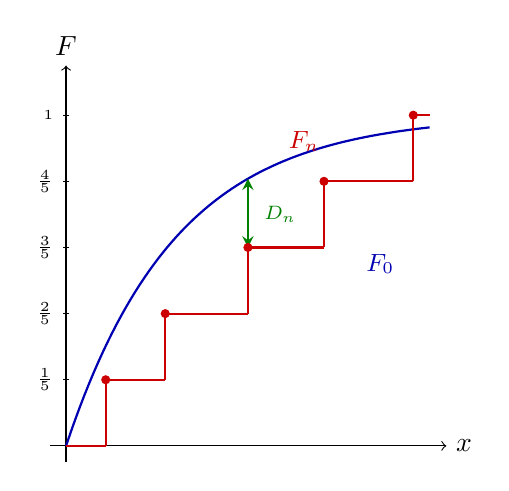
\begin{tikzpicture}[scale=4.2]
  \draw[->](-0.05,0)--(1.15,0)node[right]{$x$};
  \draw[->](0,-0.05)--(0,1.15)node[above]{$F$};
  \foreach \y/\lab in {0.2/$\tfrac{1}{5}$,0.4/$\tfrac{2}{5}$,0.6/$\tfrac{3}{5}$,0.8/$\tfrac{4}{5}$,1.0/$1$}
    \draw(0.01,\y)--(-0.01,\y)node[left,font=\tiny]{\lab};
  \draw[blue!70!black,thick,domain=0:1.1,samples=80]plot(\x,{1-exp(-3*\x)});
  \node[blue!70!black,font=\small]at(0.95,0.55){$F_0$};
  \def\xa{0.12}\def\xb{0.30}\def\xc{0.55}\def\xd{0.78}\def\xe{1.05}
  \draw[red!80!black,thick]
    (0,0)--(\xa,0)(\xa,0)--(\xa,0.2)(\xa,0.2)--(\xb,0.2)
    (\xb,0.2)--(\xb,0.4)(\xb,0.4)--(\xc,0.4)(\xc,0.4)--(\xc,0.6)
    (\xc,0.6)--(\xd,0.6)(\xd,0.6)--(\xd,0.8)(\xd,0.8)--(\xe,0.8)
    (\xe,0.8)--(\xe,1.0)(\xe,1.0)--(1.1,1.0);
  \node[red!80!black,font=\small]at(0.72,0.92){$F_n$};
  \draw[<->,>=stealth,thick,green!50!black](0.55,0.6)--(0.55,0.808);
  \node[green!50!black,font=\scriptsize,right]at(0.57,0.70){$D_n$};
  \foreach \xi/\yi in {\xa/0.2,\xb/0.4,\xc/0.6,\xd/0.8,\xe/1.0}
    \filldraw[red!80!black](\xi,\yi)circle(0.012);
\end{tikzpicture}
\end{center}
\begin{center}\small\textit{Staircase $F_n$ (red) vs.\ $F_0$ (blue). Arrow marks $D_n$.}\end{center}

% ---- 7.4 Two regimes ----
\subsection{Two Decision Regimes}

\textbf{Small samples ($n\lesssim 40$) --- exact table.}
Look up $D_{n,\alpha}$ and reject $H_0$ if $D_n > D_{n,\alpha}$.
No $\sqrt{n}$ scaling. The table exists because $G_n$ is universal.

\begin{center}
\begin{tabular}{ccccc}
\toprule
$n$ & $\alpha=0.20$ & $\alpha=0.10$ & $\alpha=0.05$ & $\alpha=0.01$ \\
\midrule
 5 & 0.447 & 0.509 & 0.565 & 0.669 \\
10 & 0.323 & 0.369 & 0.409 & 0.486 \\
20 & 0.232 & 0.265 & 0.294 & 0.352 \\
40 & 0.165 & 0.189 & 0.210 & 0.252 \\
\bottomrule
\end{tabular}
\end{center}

\textbf{Large samples ($n\gtrsim 40$) --- Kolmogorov asymptotics.}
Form $T=\sqrt{n}\,D_n$ and reject if $T>c_\alpha$, or compute
$p = P(K\geq T)= 2\sum_{k=1}^{\infty}(-1)^{k-1}e^{-2k^2T^2}$
(one term suffices for $T\geq 1.2$).

\begin{center}
\begin{tabular}{ccc}
\toprule
$\alpha$ & $c_\alpha$ & Reject if $\sqrt{n}\,D_n>$ \\
\midrule
0.10 & 1.224 & 1.224 \\
0.05 & 1.358 & 1.358 \\
0.01 & 1.628 & 1.628 \\
\bottomrule
\end{tabular}
\end{center}

% ---- 7.5 Worked example ----
\subsection{Worked Example}

\textbf{Setup.} $H_0\colon F_0=\mathrm{Exp}(1)$, so $F_0(x)=1-e^{-x}$.

\subsubsection*{Path A: $n=10$ (exact table)}

Sorted mock data: $0.11,\ 0.28,\ 0.43,\ 0.57,\ 0.74,\ 0.95,\ 1.21,\ 1.58,\ 2.03,\ 2.87$.

\begin{center}
\begin{tabular}{ccccr}
\toprule
$i$ & $x_{(i)}$ & $F_n=i/10$ & $F_0(x_{(i)})$ & $|F_n-F_0|$ \\
\midrule
1  & 0.11 & 0.10 & 0.104 & 0.004 \\
2  & 0.28 & 0.20 & 0.244 & 0.044 \\
3  & 0.43 & 0.30 & 0.349 & 0.051 \\
4  & 0.57 & 0.40 & 0.435 & 0.035 \\
5  & 0.74 & 0.50 & 0.523 & 0.023 \\
6  & 0.95 & 0.60 & 0.613 & 0.013 \\
7  & 1.21 & 0.70 & 0.702 & 0.002 \\
8  & 1.58 & 0.80 & 0.794 & 0.006 \\
9  & 2.03 & 0.90 & 0.869 & 0.031 \\
10 & 2.87 & 1.00 & 0.943 & 0.057 \\
\bottomrule
\end{tabular}
\end{center}

$D_{10}=0.057$. From exact table: $D_{10,\,0.05}=0.409$.
Since $0.057<0.409$: \textbf{fail to reject} $H_0$.

\subsubsection*{Path B: $n=100$ (Kolmogorov asymptotics)}

Mock: $D_{100}=0.121$. Scaled: $T=\sqrt{100}\cdot 0.121=1.21$.
Since $T\geq 1.2$, one term: $p\approx 2e^{-2(1.21)^2}=0.107$.
Since $T=1.21<c_{0.05}=1.358$: \textbf{fail to reject} $H_0$.
If instead $D_{100}=0.148$, then $T=1.48>1.358$: \textbf{reject}.

% ---- 7.6 Simulation ----
\subsection{Simulation Code (Python)}

\begin{verbatim}
def empirical_cdf(sample):
    n = len(sample)
    @np.vectorize
    def Fn(x): return (1/n) * np.sum(sample <= x)
    return Fn

def KS_stat(sample, F):           # returns sqrt(n)*D_n
    n = len(sample);  Fn = empirical_cdf(sample)
    grid = np.arange(np.min(sample)-1, np.max(sample)+1, 0.01)
    return np.sqrt(n) * np.max(np.abs(Fn(grid) - F(grid)))

def Brownian_bridge(t):           # B_t = W_t - t*W_1
    W = np.cumsum(np.sqrt(np.diff(t)) * nr.normal(0,1,len(t)-1))
    W = np.r_[0, W]
    return W - W[-1] * t

def KS_rv():                      # one draw of K = sup|B_t|
    return np.max(np.abs(Brownian_bridge(np.arange(0, 1, 1e-5))))

def KS_cdf():                     # empirical KS CDF from 10,000 paths
    return empirical_cdf(np.array([KS_rv() for _ in range(10000)]))
\end{verbatim}

The simulation confirms the distribution-free property in its full strength: for every
fixed $n$, the distribution of $D_n$ is \emph{exactly the same} regardless of whether
the data are Normal, Exponential, or any other continuous distribution.
The Kolmogorov distribution $G$ is only the \emph{limit} of $G_n$ as $n\to\infty$;
the universality of $G_n$ at each finite $n$ is the deeper fact, and it is what makes
the exact small-sample tables possible.

\medskip
The full runnable notebook --- with the same functions extended for typing and
reproducibility, plots of the empirical and theoretical CDFs, the simulated
KS distribution, and convergence diagnostics at $n=10, 100, 1000$ --- is at
\url{https://github.com/borisgarbuzov/notes/blob/main/KS_test.ipynb}.

%=============================================================
\section{Quick Reference: Diagnostic Tests}
%=============================================================

\begin{center}
\begin{tabular}{lll}
\toprule
\textbf{Assumption} & \textbf{Test / Method} & \textbf{What to check} \\
\midrule
Linearity & Scatter plot, residual vs.\ fitted & Visual pattern \\
Multicollinearity & VIF & VIF $> 10$ \\
Autocorrelation & Durbin-Watson & $DW \approx 2$ \\
Zero mean of residuals & One-sample $t$-test & $p > 0.05$ \\
Normality of residuals & KS test, Shapiro-Wilk, Q-Q & $p > 0.05$ \\
Homoscedasticity & Breusch-Pagan & $p > 0.05$ \\
Population stability & PSI & PSI $< 0.1$ stable, $> 0.25$ unstable \\
Discrimination (credit) & Gini / AUC, KS stat & Gini $> 0.3$ acceptable \\
\bottomrule
\end{tabular}
\end{center}

\end{document}
